%\documentclass[fullscreen=true, bookmarks=false]{beamer}
\documentclass[pdf, 12pt, unicode]{beamer}
\usepackage[cp1251]{inputenc}
\usepackage[english]{babel}
\usepackage{xcolor}
%\usetheme{Warsaw}
\usetheme{Boadilla}
\usepackage{epsfig}
\usepackage{mathtools}
\usepackage{bbm}

\newcommand{\argmin}{\mathop{argmin}}

\newcommand{\x}{\mathbf{x}}
\newcommand{\X}{\mathbf{X}}
\newcommand{\D}{\mathcal{D}}
\newcommand{\R}{\mathbb{R}}
\newcommand{\E}{\mathbb{E}}
\newcommand{\V}{\mathbb{V}}
%\newcommand{\argmin}{\mathop{argmin}}

\usepackage[ruled,vlined]{algorithm2e}

\DeclareMathOperator{\Bin}{Bin}
\DeclareMathOperator{\vol}{vol}

\newcommand{\1}{\mathbbm{1}}



\usecolortheme[rgb={0.011,0.24,0.53}]{structure}

\usepackage{tikz}
\usetikzlibrary{arrows,shapes,positioning}

\setbeamerfont{institute}{size=\normalsize}

\tikzstyle{format} = [ thick,
                      minimum size=1cm,
                      draw=white!30!black!70,
                      top color=white,
                      bottom color=blue!70!white!30,
                      font=\itshape]

\tikzstyle{empty} = [ rectangle,
                      minimum size=1cm,
                      font=\itshape]

\usepackage{tabularx}
\usepackage{multicol}
\usepackage{xcolor}

\usepackage[T2A]{fontenc}
\usepackage[cp1251]{inputenc}
\usepackage{graphicx}
\usepackage{amssymb}
\usepackage{amsthm}



\usefonttheme[onlymath]{serif}

\title[CatBoost]{CatBoost: unbiased boosting \\ with categorical features}
\author[Liudmila Prokhorenkova et al.]{Liudmila Prokhorenkova, Gleb Gusev, Aleksandr  Vorobev, \\ Anna Veronika  Dorogush, Andrey  Gulin}

\date[]{Accepted to NIPS 2018}

\begin{document}

\begin{frame}
\transdissolve[duration=0.2]
\titlepage
\end{frame}

\begin{frame}{CatBoost}
	
\begin{itemize}
\item A variant of GBDT
\item Effectively handles categorical features
\item Shows best results on many datasets (compared with MatrixNet, XGBoost, LightGBM)
\item Available as an open-source library: \url{https://github.com/catboost/}
\end{itemize}
\end{frame}

\begin{frame}{Notation}
\begin{itemize}
	\item Dataset $\D=\{(\x_k,y_k)\}_{k=1..n}$, $\x_k\in \R^m$, $y_k\in \R$ 
	\item $(\x_k,y_k)$ -- i.i.d. from $P(\cdot,\cdot)$
	\pause
	\item Looking for  $F = \mathrm{argmin}_f \, \mathcal{L}(f),\,  \,\mathcal{L}(f) := \E(L(y, f(\x)))$
	\pause
	\item Gradient boosting: $F^{t}=F^{t-1}+ \alpha^t h^{t}$,\\ 
	$h^t = \mathrm{argmin}_{h\in H} \mathcal{L}(F^{t-1}+h)$ \,\,\, (details later)
	\pause
	\item In CatBoost, $H$ is a family of oblivious decision trees with limited depth
\end{itemize}
	
\end{frame}

\begin{frame}{Categorical features}
\begin{itemize}
	\item Have discrete set of values (categories), not comparable with each other
	\item Cannot be used in binary decision trees directly
	\pause
	\item \textbf{One-hot encoding:} add binary variables identifying categories
	\item Problems: large memory requirements and computational cost, weak features
	\pause
	\item Solution: use \textit{target-based statistics} (TBS) instead
	\item We replace category $x_{k}^{i}$ by some numerical value $\hat x_{k}^{i}$
\end{itemize}
\end{frame}



\begin{frame}{Greedy TBS} 

$$
\hat x_{k}^{i} = 
\frac{\sum_{j=1}^n{ \1_{\{x_{j}^{i}=x_{k}^{i}\}}\cdot y_j}}{\sum_{j=1}^n \1_{\{x_{j}^{i}=x_{k}^{i}\}}}
$$

\pause
\-

\textbf{Problem:} target leakage leads to a conditional shift, i.e., 
$\hat x^{i}|y$  differs for training and test examples

\-

\begin{itemize}
	\item[P1] \textit{$\E(\hat x^i|y=v)$ = $\E(\hat x_k^i |y_k=v)$, where $(x_k,y_k)$ is the $k$-th training example}
\end{itemize}

\pause 
\-

\textbf{Example:} $i$-th feature is categorical, all values are unique, $P(y=1|x^i=a) = 0.5$:
$$\E(\hat x_k^i |y_k) = y_k\in\{0,1\}$$  
$$\E(\hat x^i|y) = 0.5$$

\end{frame}

\begin{frame}{Greedy TBS with prior}


$$
\hat x_{k}^{i} = \frac{\sum_{j=1}^n{\1_{\{x_{j}^{i}=x_{k}^{i}\}}\cdot y_j}+a\,P}{\sum_{j=1}^n\1_{\{x_{j}^{i}=x_{k}^{i}\}}+a}
$$

\pause
\-

Still problems with P1:  \\
$\hat x_{k}^{i} = \frac{aP}{1+a}$ if $y_k=0$ \\
$\hat x_{k}^{i} =\frac{1+aP}{1+a}$ if $y_k=1$ 

\end{frame}

\begin{frame}{Holdout TBS}

General approach:
$$
\hat x_{k}^{i} = \frac{\sum_{\x_j \in \D_k}{\1_{\{x_{j}^{i}=x_{k}^{i}\}}\cdot y_j}+a\,P}{\sum_{\x_j \in \D_k}\1_{\{x_{j}^{i}=x_{k}^{i}\}}+a}
$$

\pause
\-

\textit{Holdout TBS}: $\D = \hat \D_0 \sqcup \hat \D_1$, use $\D_k = \hat \D_0$ to calculate the TBS and $\hat \D_1$ to perform training

\-
\pause

\begin{itemize}
	\item[P2] \textit{It is desirable for $\hat x_{k}^{i}$ to have a low variance}
\end{itemize}

\end{frame}

\begin{frame}{Leave-one-out TBS} 

\begin{itemize}
\item $\D_k = \D \setminus \x_k$ for training examples and $\D_k = \D$ for test examples
\pause
\item \textbf{Example:} $x_k^i = a$ for all examples \\
Let $n^+$ be the number of examples with $y=1$ \\ 
$\hat x_{k}^{i} = \frac{n^+ - y_k + a\,P}{n - 1 + a}$\\
\pause
\item For a test example: $\hat x^{i} = \frac{n^+ + a\,P}{n + a}$ 
\end{itemize}

\end{frame}



\begin{frame}{Ordered TBS}

\begin{itemize}
\item Perform a random permutation $\sigma$ of the dataset
\item Take $\D_k = \{\x_j:\sigma(j)<\sigma(k)$\} for a training example $\x_k$ and $\D_k = \D$ for a test example
\pause
\item Obtained \textit{ordered} TBS satisfies the requirement P1, and we also reduce the variance of $\hat x^i_k$ (see P2) compared to sliding window TBS used in online learning
\item CatBoost uses several permutations
\end{itemize}
\end{frame}


\begin{frame}{Comparison of TBS}

Relative change in logloss / zero-one loss:

\begin{figure}
	\centering
	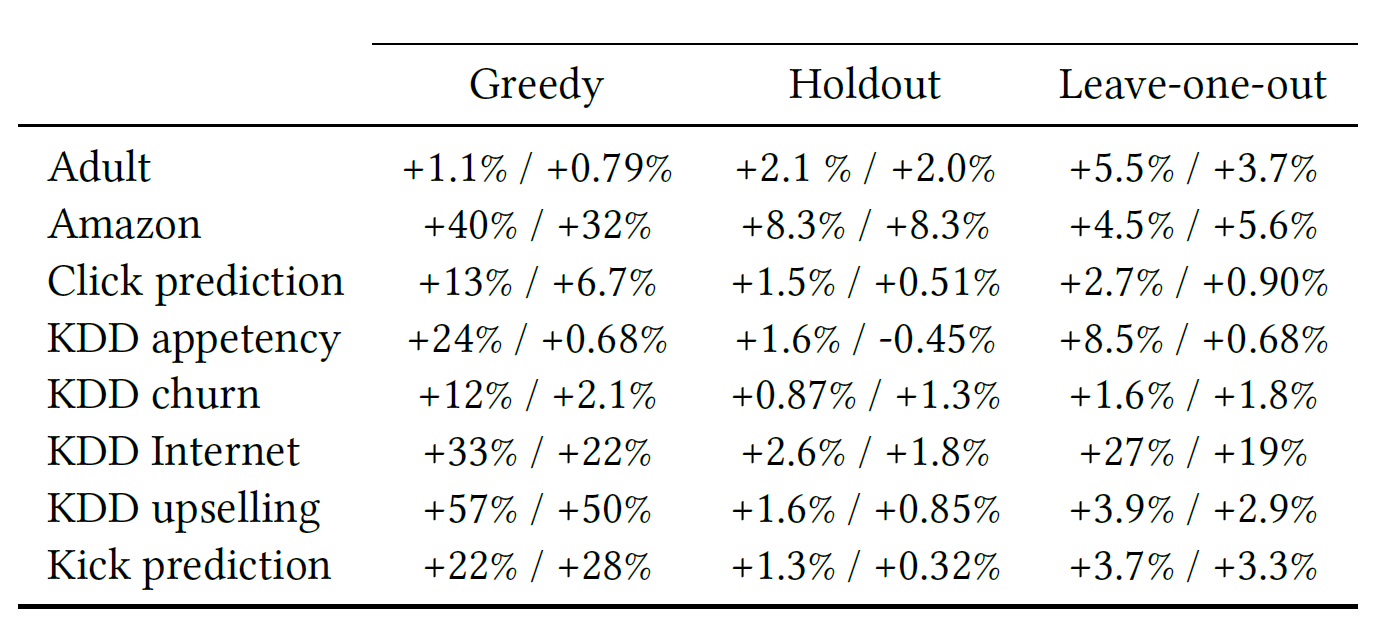
\includegraphics[width=\textwidth]{tbs.png}
\end{figure}


\end{frame}

\begin{frame}{Prediction shift}

\begin{itemize}
	\item Gradient boosting: $F^{t}=F^{t-1}+ \alpha^t h^{t}$,\\ 
	$h^t = \mathrm{argmin}_{h\in H} \mathcal{L}(F^{t-1}+h)$ \,\,\, 
	\pause  
	\item $g^t(\x,y):=\frac{\partial L(y,s)}{\partial s}\big|_{s=F^{t-1}(\x)}$
	\item $\hat h^t = \mathrm{argmin}_{h\in H} \E\left (-g^t(\x,y)- h(\x)\right )^2$ 
	\pause
	\item $ h^t = \mathrm{argmin}_{h\in H} \frac{1}{n}\sum_{k=1}^{n} \left (-g^t(\x_k, y_k) -  h(\x_k)\right )^2$
\end{itemize}

\pause

Shifts:
\begin{enumerate}
	\item $g^t(\x_k, y_k)\mid \x_k$ is shifted from $g^t(\x, y)\mid \x$
	\item So, $h^t$ is biased with respect to $\hat h^t$
	\item This, finally, affects the generalization ability of the trained model $F^t$
\end{enumerate}

\end{frame}

\begin{frame}{Theoretical example}
	
\begin{itemize}
\item Two features $x^1, x^2$~--- i.i.d. Bernoulli random variables with $p = 1/2$
\item $y=f^*(\x)=c_1x^1+c_2x^2$
\item Use decision stumps, $\alpha = 1$, $N=2$
\item $F^2=h^1+h^2$, $h^1$ based on $x^1$ and $h^2$ based on $x^2$ 
\end{itemize}

\pause

\begin{block}{Proposition}
	\begin{enumerate}
		\item If two independent samples $\D_1$ and $\D_2$ of size $n$ are used to estimate $h^1$ and $h^2$, respectively, then
		$\E_{\D_1, \D_2} F^2(\x)=f^*(\x)+O(1/2^{n})$ for any $\x\in \{0,1\}^2$.
		\item If the same dataset $\D$ is used for both $h^1$ and $h^2$, then $\E_{\D_1, \D_2} F^2(\x)=f^*(\x)-\frac{1}{n-1}c_2(x^2-\frac{1}{2})+O(1/2^{n})$.
	\end{enumerate}
\end{block}


\end{frame}



\begin{frame}{Ordered boosting}

\begin{figure}
	\centering
	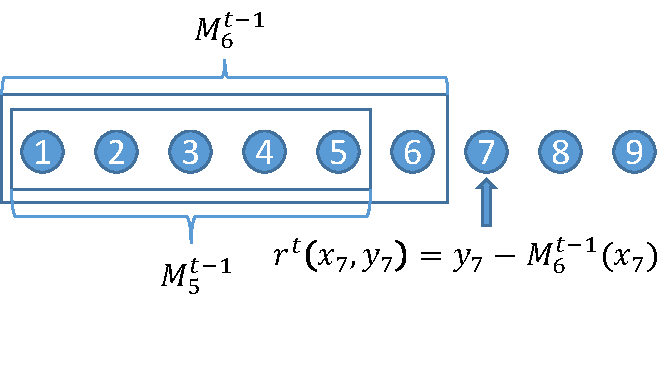
\includegraphics[width=\textwidth]{comics.pdf}
\end{figure}

\end{frame}


\begin{frame}{Ordered boosting}


\begin{figure}
	\centering
	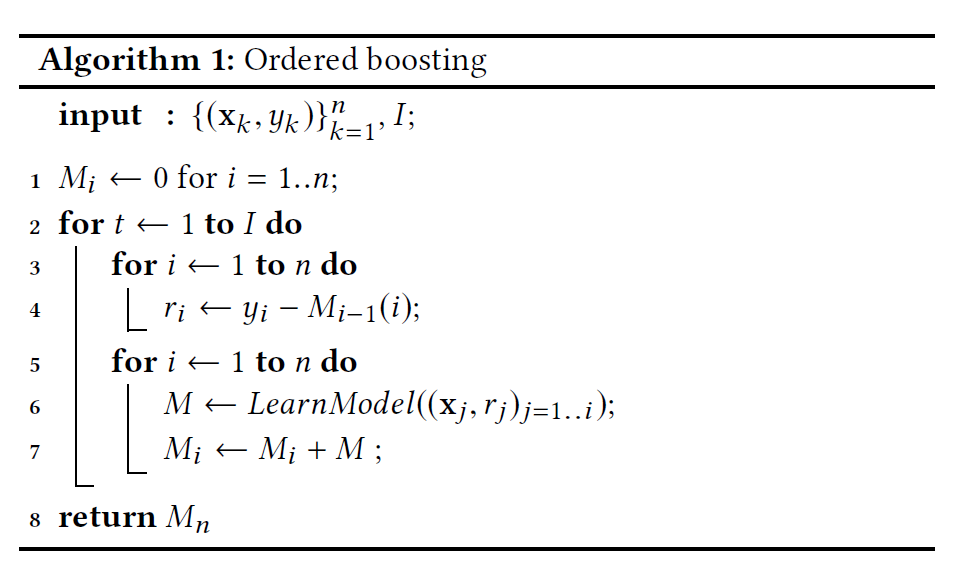
\includegraphics[width=\textwidth]{algorithm.png}
\end{figure}

\end{frame}

	




\begin{frame}{Implementation}

Two phases: choosing the tree structure and choosing the values in leaves

\-

Second phase:
\begin{itemize}
\item This phase uses the standard GBDT scheme 
\item $\sigma_0$~--- random permutation used for computing ordered TBS
\end{itemize}

\-
\pause

First phase:
\begin{itemize}
	\item Two modes: \textit{Ordered} and \textit{Plain}
	\item $\sigma_1, \ldots, \sigma_s$~--- random permutation used for computing ordered TBS, also used in Ordered mode
	\item At each step we construct a tree based on a randomly sampled permutation $\sigma_r$
\end{itemize}

\end{frame}

\begin{frame}{Implementation}

Ordered mode:
\begin{itemize}
	\item For simplicity of notation order examples according to $\sigma_r$
	\item $S_{r,j}(i)$~--- current prediction for $i$-th example based on examples $1..j$
	\item $grad_{r,j}(i)$ is computed based on $S_{r,j}(i)$
	\pause
	\item Target gradient: $G = (grad_{r,0}(1), \ldots, grad_{r,n-1}(n))$
	\item Choosing a split: for $i$-th example average $grad_{r,i-1}(j)$ for $j<i$ in the same leaf and compare the obtained vector with $G$
	\pause
	\item $S_{r,j}(i) \leftarrow S_{r,j}(i) - \alpha \, \mathrm{avg}(grad_{r,i-1}(j) \text{ for } j<i \text{ in the same leaf})$
\end{itemize}

\end{frame}


\begin{frame}{Comparison with baselines}

Logloss / zero-one loss, relative increase is presented in the brackets:

	\begin{figure}
		\centering
		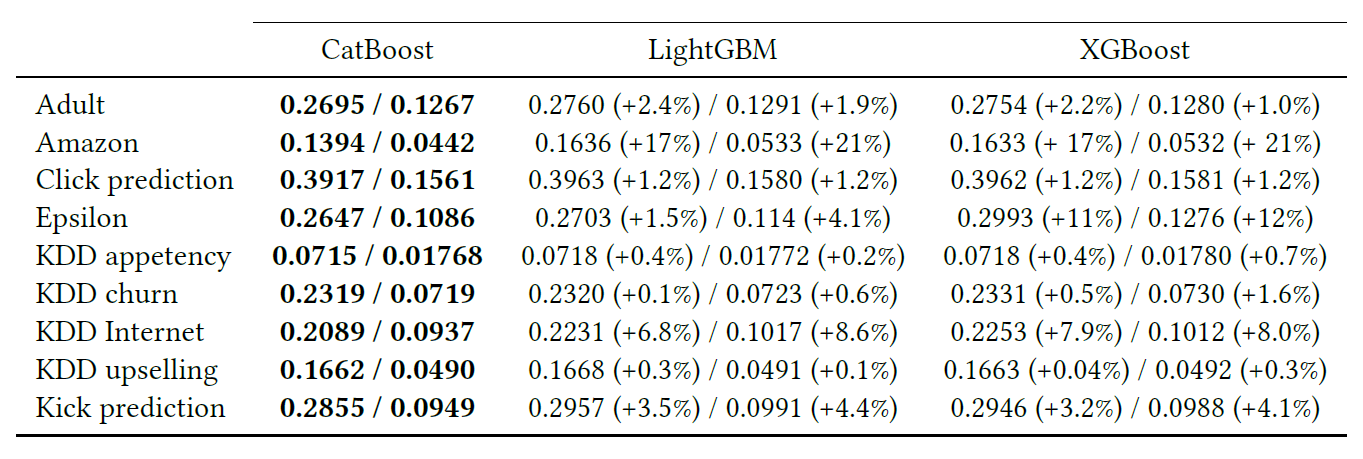
\includegraphics[width=\textwidth]{baselines.png}
	\end{figure}

\end{frame}

\begin{frame}{Ordered vs Plain}
\begin{small}
	\begin{table}
		\caption{Plain mode: logloss, zero-one loss and their relative change compared to Ordered mode}\label{tab:plain}
		\centering
		\begin{tabular}{l|cc}
			& Logloss &  Zero-one loss \\
			%\midrule
			\hline
			Adult & 
			0.2723 (+1.1\%) &
			0.1265	(-0.1\%) \\
			Amazon & 
			0.1385 (-0.6\%) & 
			0.0435	(-1.5\%) \\	
			Click prediction & 
			0.3915	(-0.05\%) & 
			0.1564	(+0.19\%) \\
			Epsilon & 
			0.2663 (+0.6\%) & 
			0.1096 (+0.9\%) \\
			KDD appetency & 
			0.0718	(+0.5\%) & 
			0.0179	(+1.5\%) \\
			Kdd churn & 
			0.2317	(-0.06\%) & 
			0.0717	(-0.17\%)  \\
			KDD internet & 
			0.2170 (+3.9\%) & 
			0.0987 (+5.4\%) \\
			KDD upselling & 
			0.1664 (+0.1\%) & 
			0.0492 (+0.4\%) \\
			Kick prediction & 
			0.2850 (-0.2\%) & 
			0.0948 (-0.1\%) \\
		\end{tabular}
	\end{table}
\end{small}

\end{frame}

\begin{frame}{Ordered vs Plain, effect of size}

\begin{figure}
	\centering
	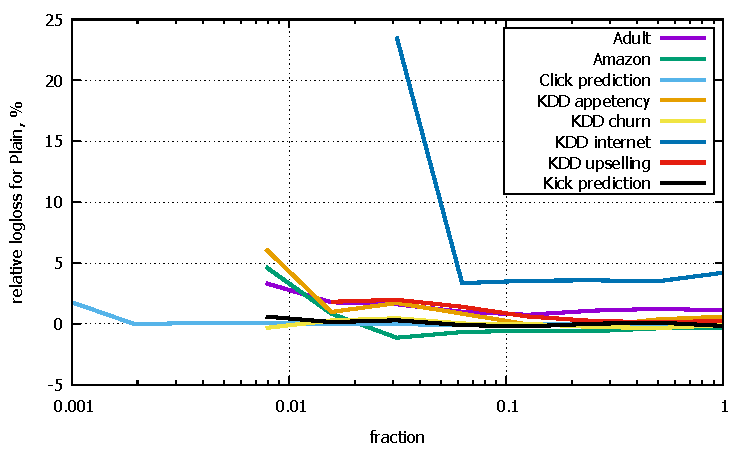
\includegraphics[width=0.8\textwidth]{plain_logloss.pdf}
	%\includegraphics[width=0.49\textwidth]{plain_error.pdf}
	\caption{Relative error of Plain compared to Ordered depending on the fraction of the dataset}\label{fig:plain_filtered}
\end{figure}

\end{frame}
	
\begin{frame}{Feature combinations}
\begin{figure}
	\centering
	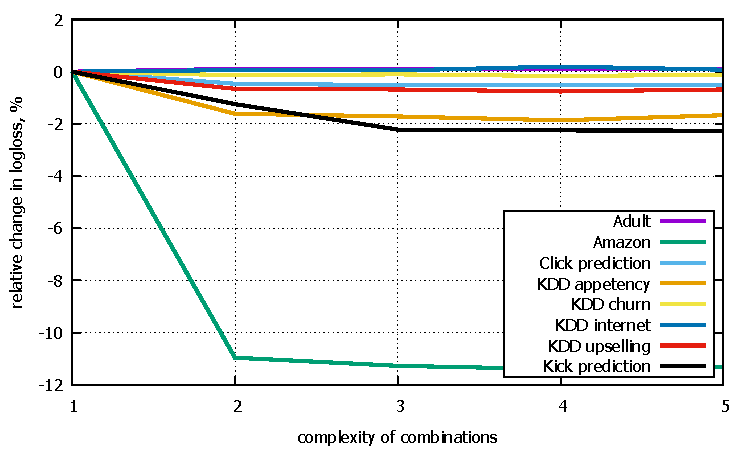
\includegraphics[width=0.8\textwidth]{complexity_logloss.pdf}
	\caption{Relative change in logloss for a given allowed complexity compared to the absence of combinations}\label{fig:combinations}
\end{figure}
\end{frame}
	
\begin{frame}{Number of permutations}
\begin{figure}
	\centering
	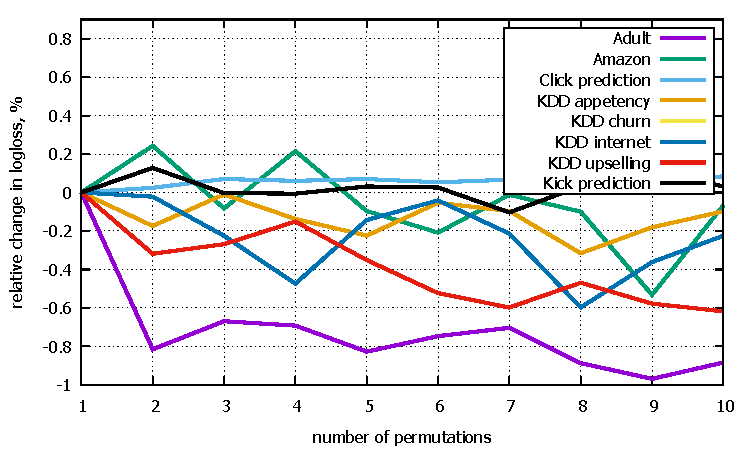
\includegraphics[width=0.8\textwidth]{folds_logloss.pdf}
	\caption{Relative change in logloss for a given number of permutations $s$ compared to $s=1$}\label{fig:folds}
\end{figure}
\end{frame}




\end{document}

